\documentclass{mwart}\usepackage[]{graphicx}\usepackage[]{xcolor}
% maxwidth is the original width if it is less than linewidth
% otherwise use linewidth (to make sure the graphics do not exceed the margin)
\makeatletter
\def\maxwidth{ %
  \ifdim\Gin@nat@width>\linewidth
    \linewidth
  \else
    \Gin@nat@width
  \fi
}
\makeatother

\definecolor{fgcolor}{rgb}{0.345, 0.345, 0.345}
\newcommand{\hlnum}[1]{\textcolor[rgb]{0.686,0.059,0.569}{#1}}%
\newcommand{\hlstr}[1]{\textcolor[rgb]{0.192,0.494,0.8}{#1}}%
\newcommand{\hlcom}[1]{\textcolor[rgb]{0.678,0.584,0.686}{\textit{#1}}}%
\newcommand{\hlopt}[1]{\textcolor[rgb]{0,0,0}{#1}}%
\newcommand{\hlstd}[1]{\textcolor[rgb]{0.345,0.345,0.345}{#1}}%
\newcommand{\hlkwa}[1]{\textcolor[rgb]{0.161,0.373,0.58}{\textbf{#1}}}%
\newcommand{\hlkwb}[1]{\textcolor[rgb]{0.69,0.353,0.396}{#1}}%
\newcommand{\hlkwc}[1]{\textcolor[rgb]{0.333,0.667,0.333}{#1}}%
\newcommand{\hlkwd}[1]{\textcolor[rgb]{0.737,0.353,0.396}{\textbf{#1}}}%
\let\hlipl\hlkwb

\usepackage{framed}
\makeatletter
\newenvironment{kframe}{%
 \def\at@end@of@kframe{}%
 \ifinner\ifhmode%
  \def\at@end@of@kframe{\end{minipage}}%
  \begin{minipage}{\columnwidth}%
 \fi\fi%
 \def\FrameCommand##1{\hskip\@totalleftmargin \hskip-\fboxsep
 \colorbox{shadecolor}{##1}\hskip-\fboxsep
     % There is no \\@totalrightmargin, so:
     \hskip-\linewidth \hskip-\@totalleftmargin \hskip\columnwidth}%
 \MakeFramed {\advance\hsize-\width
   \@totalleftmargin\z@ \linewidth\hsize
   \@setminipage}}%
 {\par\unskip\endMakeFramed%
 \at@end@of@kframe}
\makeatother

\definecolor{shadecolor}{rgb}{.97, .97, .97}
\definecolor{messagecolor}{rgb}{0, 0, 0}
\definecolor{warningcolor}{rgb}{1, 0, 1}
\definecolor{errorcolor}{rgb}{1, 0, 0}
\newenvironment{knitrout}{}{} % an empty environment to be redefined in TeX

\usepackage{amsmath}
\usepackage{alltt}


\usepackage[utf8]{inputenc}
\usepackage[T1]{fontenc}
\usepackage{lmodern}
\usepackage{microtype}
\usepackage[breaklinks, hidelinks, pdfusetitle, pdfdisplaydoctitle]{hyperref}
\usepackage{icomma}
\usepackage{booktabs}
\usepackage[locale=DE]{siunitx}
\usepackage{placeins}
\usepackage{polski}


\author {
    Kacper Budnik
    \and
    Eryka Grygutis
    \and
    Karolina Jonczyk
    \and
    Jakub Kaczor
}
\title {Projekt bazy danych}
\date \today
\IfFileExists{upquote.sty}{\usepackage{upquote}}{}
\begin{document}
\maketitle



\section*{Wprowadzenie}
W tej analizie odpowiemy kolejno na następujące pytania, dotyczące bazy
danych klubu sportowego Curling Masters.
\begin{enumerate}
    \item Jak wygląda rozkład spotkań ze względu na miesiąc?
    \item Jaki procent graczy w historii brał udział w grach?
    \item Jak wygląda ranking najlepszych 10 graczy w historii klubu?
    \item Jak się ma stosunek wygranych do przegranych ze względu na
        sekcje?
    \item Czy w okolicy turniejów, sprzęt w wypożyczalni cieszy się
        większym popytem?
    \item Czy w wypożyczalni klubu, ilość sprzętu jest wystarczająca?
\end{enumerate}
\begin{knitrout}
\definecolor{shadecolor}{rgb}{0.969, 0.969, 0.969}\color{fgcolor}\begin{figure}
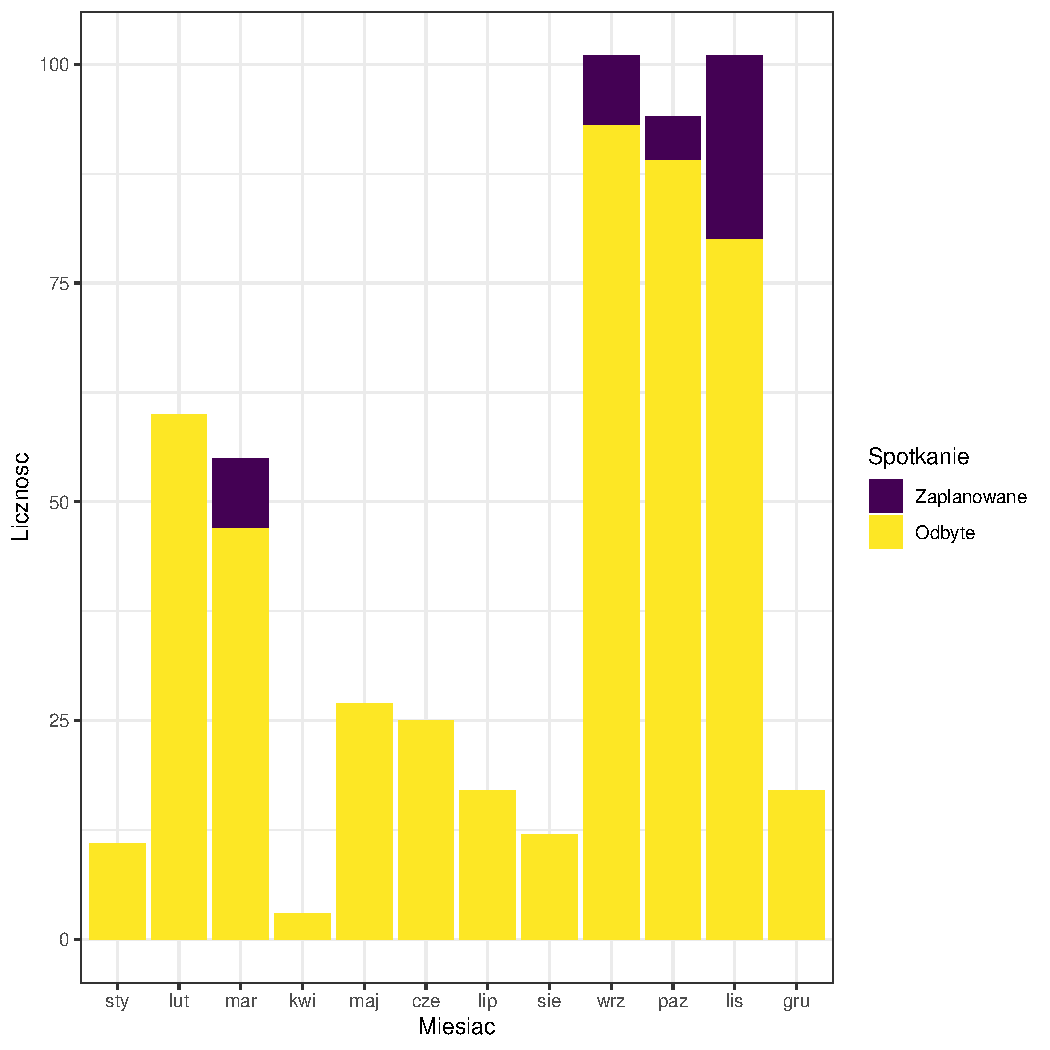
\includegraphics[width=\maxwidth]{figure/unnamed-chunk-2-1} \caption[Rozkład odbytych gier ze względu na miesiąc roku]{Rozkład odbytych gier ze względu na miesiąc roku.}\label{fig:unnamed-chunk-2}
\end{figure}

\end{knitrout}
\begin{knitrout}
\definecolor{shadecolor}{rgb}{0.969, 0.969, 0.969}\color{fgcolor}\begin{figure}
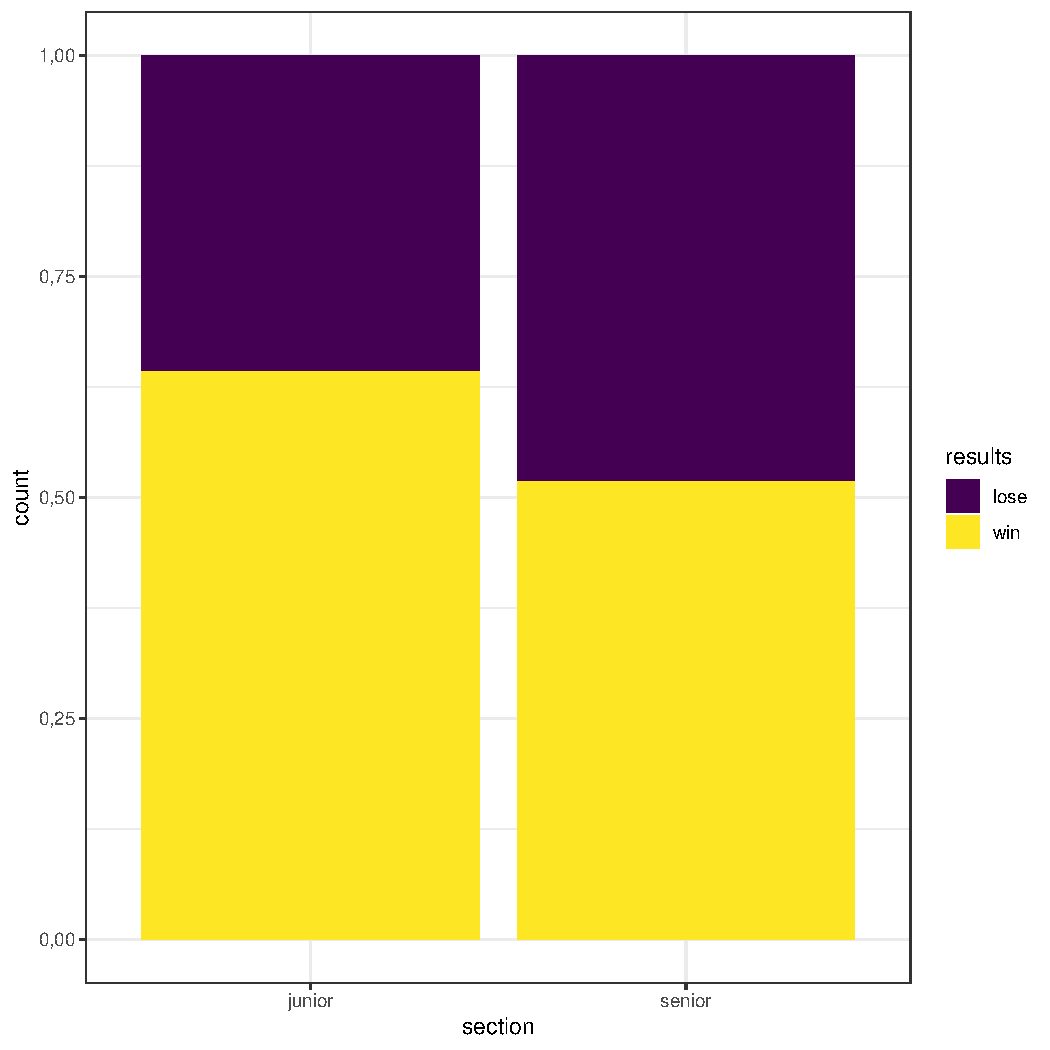
\includegraphics[width=\maxwidth]{figure/unnamed-chunk-3-1} \caption[Bilans wygranych i przegranych ze względu na sekcję]{Bilans wygranych i przegranych ze względu na sekcję.}\label{fig:unnamed-chunk-3}
\end{figure}

\end{knitrout}
\section {Jak wygląda rozkład spotkań ze względu na miesiąc?}

Zgodnie z histogramem przedstawionym na rysunku 1. najwięcej meczy rozegrano kolejno w lutym, październiku i wrześniu. W 6 miesiącach (luty, marzec, sierpień, wrzesień, październik i listopad) zaplanowano więcej meczy niż zostały rozegrane. To oznacza, że podczas sezonu rozgrywek zawsze zaplanowano o kilka spotkań więcej. Kwiecień był miesiącem, w którym rozegrano najmniej meczy. Uważnie przyglądając się wykresowi, można stwierdzić, że największe natężenie rozgrywek przypada na końcówkę zimy (luty, marzec) oraz jesień (wrzesień, październik, listopad). 

%RYSUNEK 1, RYSUNEK 3

\begin{knitrout}
\definecolor{shadecolor}{rgb}{0.969, 0.969, 0.969}\color{fgcolor}\begin{kframe}


{\ttfamily\noindent\bfseries\color{errorcolor}{\#\# Error: <text>:32:2: nieoczekiwany symbol\\\#\# 31: ) * 100\\\#\# 32: \textbackslash{}section\\\#\# \ \ \ \ \ \textasciicircum{}}}\end{kframe}
\end{knitrout}

Nie każdy członek klubu rozegrał chociaż jeden mecz. Okazuje się, że spośród wszystkich 60 graczy, tylko 17 brało udział w odbytych grach. Jest to ok. 28,3 \% wszystkich graczy. Oznacza to, że na rozgrywki zostaje wystawiana pewna grupa klubowiczów. Możemy wnioskować, że to są najlepsi gracze z klubu.
%Okazuje się, że spośród wszystkich all_players_count graczy, tylko
%participated_players_count brało udział w odbytych grach. Jest to
%ok. participation_percentage\,\%. W takim wypadku nie
%będziemy używać wyszukanych sposobów na znalezienie formuły oceny,
%a jedynie odfiltrujemy przypadki typu 0/1 oraz 1/1. Powiedzmy, że za poziom
%istotności stosunku wygranych do przegranych ustalamy na minimum 40
%rozegranych gier. Wtedy ranking najlepszych graczy wygląda tak, jak
%w tabeli \ref{tab:ranking}.

\begin{knitrout}
\definecolor{shadecolor}{rgb}{0.969, 0.969, 0.969}\color{fgcolor}\begin{kframe}


{\ttfamily\noindent\bfseries\color{errorcolor}{\#\# Error in filter(., !is.na(win\_ratio), count >= 40): nie znaleziono obiektu 'results'}}

{\ttfamily\noindent\bfseries\color{errorcolor}{\#\# Error in left\_join(., personal\_data, by = c(personal\_data\_id = "{}id"{}), : nie znaleziono obiektu 'results'}}

{\ttfamily\noindent\bfseries\color{errorcolor}{\#\# Error in arrange(., desc(win\_ratio)): nie znaleziono obiektu 'results'}}

{\ttfamily\noindent\bfseries\color{errorcolor}{\#\# Error in kable(., col.names = c("{}Imię"{}, "{}Nazwisko"{}, "{}Wygrane"{}, "{}Zagrane"{}, : nie znaleziono obiektu 'results'}}\end{kframe}
\end{knitrout}
\section{Jak wygląda ranking najlepszych 10 graczy w historii klubu?}

@
Ranking najlepszych 10 graczy w historii klubu jest zależny od procentu graczy biorących udział kiedykolwiek w meczach. Oczywiście sam stosunek wygranych do zagranych nie wystarczy. Gracze, którzy zagrali tylko jedną grę, ale wygraną, byliby według wskaźnika tymi najlepszymi. Należałoby uchwycić jeszcze pewność oceny. W takim wypadku nie będziemy używać wyszukanych sposobów na znalezienie formuły oceny, a jedynie odfiltrujemy przypadki typu 0/1 oraz 1/1. Powiedzmy, że za poziom istotności stosunku wygranych do przegranych ustalamy na minimum 40 rozegranych gier. Wtedy ranking najlepszych graczy wygląda tak, jak pokazano to poniżej w tabeli 1. Najlepszym graczem jest Michał Rekść i jego skuteczność to 70,37 \% wygranych meczy z wszystkich zagranych przez tego zawodnika.

%TABELA 1 POPRAWIONA (BEZ JĘZ POLSKIEGO IMIE, NAZWISKO ITP)
\section{Jak się ma stosunek wygranych do przegranych ze względu na sekcje?}
@
Korzystając z rysunku 2. wiadomo, że przegrane zostały oznaczone kolorem żółtym, a przegrane fioletowym. Średnio to juniorzy wygrywali częściej niż seniorzy. Skuteczność juniorów to około 65 \%, a seniorów to niewiele ponad 52 \%.

%RYSUNEK 2

\section{Czy w okolicy turniejów sprzęt w wypożyczalni cieszy się większym popytem?}

@

Omawiana baza danych uwzględnia wypożyczalnię (rental i equipment) sprzętu curlingowego dla zainteresowanych tym sportem. W wypożyczalni mamy możliwość wypożyczenia butów, szczotek, kamieni, rękawic i stoperów od 5 różnych firm. Moglibyśmy się spodziewać, że w czasie rozgrywek turniejowych ludzie są bardziej zainteresowani sportem i wypożyczają więcej sprzętu z naszej wypożyczalni. Zbadajmy taką zależność. Będziemy analizowali uśredniony rok. Pierwsze co należy zrobić, to zidentyfikować okres, w którym to odbywają się turnieje. Miesiące w których tego typu wydarzenia miały miejsce, można zobaczyć na rysunku 3. Dla tych miesięcy, mieliśmy średnio 123 wypożyczeń miesięcznie, natomiast w całym roku — 10 miesięcznie. Najczęściej wypożyczaną rzeczą były rękawiczki w rozmiarze dziecięcym. Podsumowując, w trakcie turniejów sprzęt z wypożyczalni cieszy się dużo większym zainteresowaniem.

% TABELA 2

\section{Czy w wypożyczalni klubu, ilość sprzętu jest wystarczająca? }

@
Chcielibyśmy sprawdzić, czy ilość sprzętu, jaką posiadamy, jest wystarczająca. W tym celu sprawdzimy, czy wystąpiły sytuacje, w których wypożyczony został cały sprzęt danego typu. Okazuje się, że takie sytuacje wystąpiły. Dotyczyły produktów, które znajdują się w tabeli 2 z dodatku A. Należałoby ją przejrzeć i doposażyć magazyn w kolejnym sezonie, aby uniknąć sytuacji, w których brakuje sprzętu w wypożyczalni, gdyż może to skutkować niezadowoleniem klientów (a za tym idzie ryzyko wyboru przez nich innej wypożyczalni następnym razem) oraz mniejszym zyskiem. 



\begin{knitrout}
\definecolor{shadecolor}{rgb}{0.969, 0.969, 0.969}\color{fgcolor}\begin{figure}
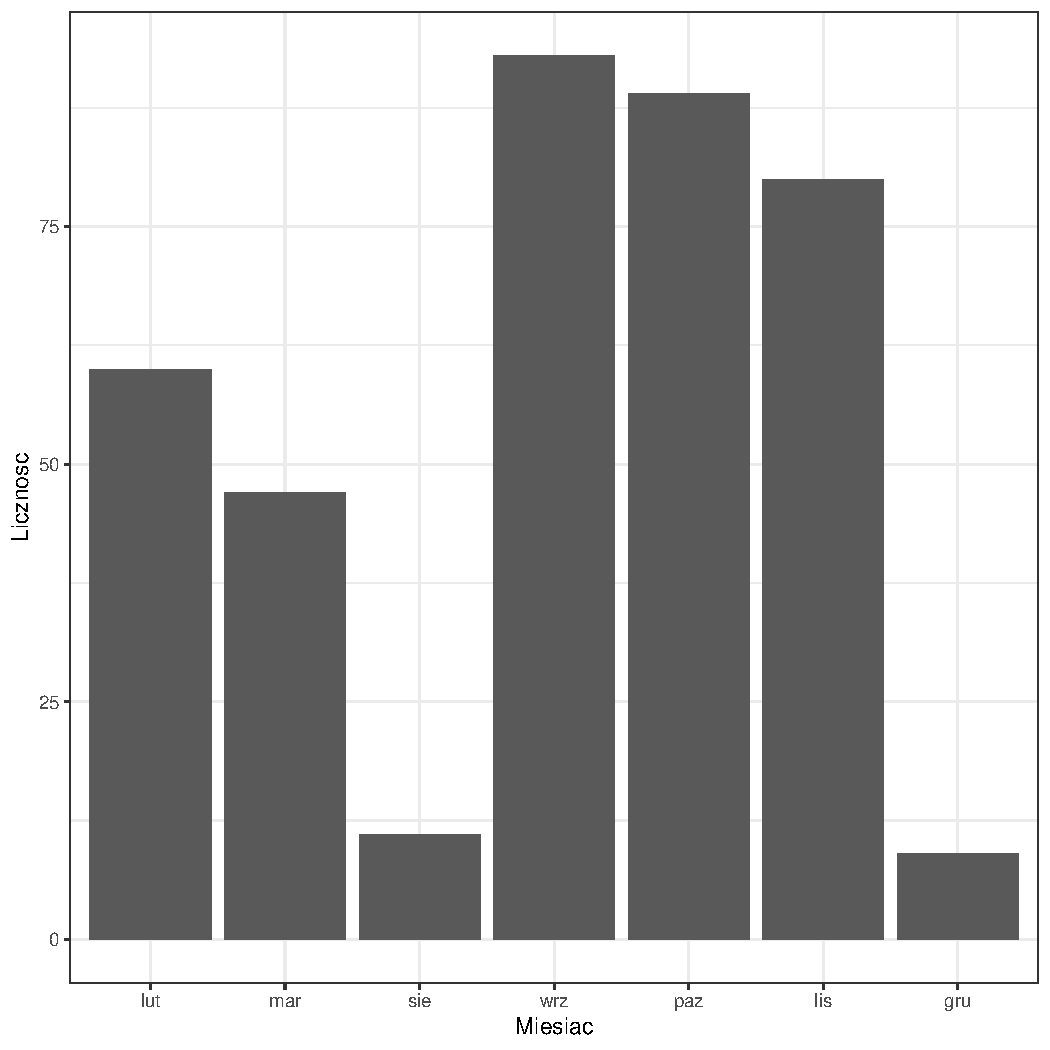
\includegraphics[width=\maxwidth]{figure/tournaments-1} \caption[Występowanie gier turniejowych ze względu na miesiąc roku]{Występowanie gier turniejowych ze względu na miesiąc roku.}\label{fig:tournaments}
\end{figure}

\end{knitrout}





\FloatBarrier
\appendix
\section {Braki w magazynie}\label {depleted}
\begin{knitrout}
\definecolor{shadecolor}{rgb}{0.969, 0.969, 0.969}\color{fgcolor}\begin{table}

\caption{\label{tab:depleted}Produkty dla których wypożyczono wszystkie egzemplarze wraz z wystąpieniami (w dniach).}
\centering
\begin{tabular}[t]{rlllr}
\toprule
id\_equipment & kind & brand & target\_group & occurences\\
\midrule
45 & gloves & balanceplus & adult & 902\\
43 & gloves & balanceplus & children & 17\\
46 & gloves & goldcurling & children & 13\\
44 & gloves & balanceplus & teeneger & 12\\
38 & shoes & asham & teeneger & 7\\
\addlinespace
40 & shoes & hardline & children & 7\\
47 & gloves & goldcurling & teeneger & 6\\
13 & stones & balanceplus & children & 4\\
26 & stones & Olson & teeneger & 4\\
31 & shoes & balanceplus & children & 4\\
\addlinespace
48 & gloves & goldcurling & adult & 4\\
52 & gloves & Olson & children & 4\\
42 & shoes & hardline & adult & 2\\
\bottomrule
\end{tabular}
\end{table}

\end{knitrout}

\end{document}
